\documentclass[12pt,a4paper]{report}

% =====================================================
% PAGE LAYOUT
% =====================================================
\usepackage[left=1.57in,top=1.18in,bottom=1in,right=1in]{geometry}
\usepackage{setspace}
\usepackage{float}
\usepackage{graphicx}
\graphicspath{{Images/}{Figures/}}
\usepackage{tocloft}

% =====================================================
% LANGUAGE & FONTS (XeLaTeX Required)
% =====================================================
\usepackage{fontspec}
\usepackage{polyglossia}

\setdefaultlanguage{english}
\setotherlanguage{bengali}

\newfontfamily\bengalifont[Script=Bengali]{Noto Serif Bengali}

% =====================================================
% MATHEMATICS
% =====================================================
\usepackage{amsmath,amssymb,mathtools}

\DeclareMathOperator*{\argmax}{arg\,max}
\DeclareMathOperator*{\argmin}{arg\,min}
\DeclarePairedDelimiter{\abs}{\lvert}{\rvert}

\newcommand{\degree}[1]{${#1}^\circ$}

% =====================================================
% TABLES & FIGURES
% =====================================================
\usepackage{booktabs}
\usepackage{array}
\usepackage{longtable}
\usepackage{tabularx}
\usepackage{multirow}
\usepackage{diagbox}

\usepackage{caption}

\captionsetup[figure]{labelfont=bf}
\captionsetup[table]{labelfont=bf}

% =====================================================
% COLORS & LISTINGS
% =====================================================
\usepackage[svgnames,table]{xcolor}
\usepackage{listings}

\definecolor{dkgreen}{rgb}{0,0.6,0}
\definecolor{gray}{rgb}{0.5,0.5,0.5}
\definecolor{mauve}{rgb}{0.58,0,0.82}

\lstset{
  frame=tb,
  language=C++,
  basicstyle=\small\ttfamily,
  keywordstyle=\color{blue},
  commentstyle=\color{dkgreen},
  stringstyle=\color{mauve},
  breaklines=true
}

% =====================================================
% ALGORITHMS
% =====================================================
\usepackage[ruled,linesnumbered]{algorithm2e}

% =====================================================
% HYPERLINKS
% =====================================================
\usepackage{hyperref}

\hypersetup{
    colorlinks=true,
    linkcolor=black,
    citecolor=black,
    urlcolor=black
}

% =====================================================
% CENTER TOC / LOF / LOT TITLES
% =====================================================
\renewcommand{\cfttoctitlefont}{\hfill\Large\bfseries}
\renewcommand{\cftaftertoctitle}{\hfill}

\renewcommand{\cftloftitlefont}{\hfill\Large\bfseries}
\renewcommand{\cftafterloftitle}{\hfill}

\renewcommand{\cftlottitlefont}{\hfill\Large\bfseries}
\renewcommand{\cftafterlottitle}{\hfill}

% =====================================================
% LIST OF FIGURES FORMAT
% =====================================================
\renewcommand{\cftfigpresnum}{Fig.\ }
\renewcommand{\cftfignumwidth}{2cm}

\addtocontents{lof}{
\protect\noindent
\protect\makebox[3cm][L]{\textbf{Fig. No.}}
\textbf{Figure Caption}
\hfill
\textbf{Page No.}
\par
}

% =====================================================
% LIST OF TABLES FORMAT
% =====================================================
\renewcommand{\cfttabpresnum}{Table\ }
\renewcommand{\cfttabnumwidth}{2cm}

\addtocontents{lot}{
\protect\noindent
\protect\makebox[3cm][L]{\textbf{Table No.}}
\textbf{Table Caption}
\hfill
\textbf{Page No.}
\par
}

% =====================================================
% FOOTER STYLE
% =====================================================
% =====================================================
% FOOTER STYLE
% =====================================================
\usepackage{fancyhdr}

% ---------- MAIN THESIS STYLE ----------
\fancypagestyle{thesis}{
    \fancyhf{}
    \renewcommand{\headrulewidth}{0pt}
    \renewcommand{\footrulewidth}{0.7pt}
    \fancyfoot[L]{\nouppercase{\leftmark}}
    \fancyfoot[R]{\thepage}
}

% ---------- FRONT MATTER STYLE ----------
\fancypagestyle{front}{
    \fancyhf{}
    \renewcommand{\headrulewidth}{0pt}
    \renewcommand{\footrulewidth}{0.7pt}
    \fancyfoot[C]{\thepage}
}

% Proper chapter mark format
\renewcommand{\chaptermark}[1]{%
    \markboth{Chapter \thechapter.\ #1}{}
}
% =====================================================
% DOCUMENT START
% =====================================================

\begin{document}

% =====================================================
% FRONT MATTER
% =====================================================
\pagestyle{front}

\fancypagestyle{plain}{
    \fancyhf{}
    \renewcommand{\headrulewidth}{0pt}
    \renewcommand{\footrulewidth}{0.7pt}
    \fancyfoot[C]{\thepage}
}

\pagenumbering{roman}
\onehalfspacing


\begin{titlepage}

\begin{center}
\Large{\textbf{Closing the Loop on RAG Hallucinations: Inference-Time Control via Dual Residual-Stream and FFN Activation Probes}\par}

\end{center}


\begin{center}
\begin{figure}[h!]
    \centering
    
\includegraphics[width=0.30\textwidth]{Images/cuet_logo.PNG}
    \label{fig:cuet_logo}
\end{figure}
\vspace{1cm}

\vspace{0.8cm}
{\large{\textit{by}}}\\
\vspace{0.8cm}
	
	{\Large{\href{https://scholar.google.com/citations?user=wObQzNsAAAAJ&hl=en}{Muhammad Junayed}}}\par 
	\vspace{.5cm}
	{\Large{2008023} }\par
	\vspace{1.5 cm}
	 This thesis is submitted in partial fulfillment of the requirement for the degree of\\
	 \textsc{BACHELOR of SCIENCE in Electronics and Telecommunication Engineering}\\
	 
\vspace{1.8 cm}

\definecolor{myblue1}{RGB}{0, 110, 255}

\par\noindent\color{Goldenrod}\rule{\textwidth}{2pt}
\large{\textcolor{blue}{Department of Electronics and Telecommunication Engineering}}\\

\large{\textbf{\textcolor{NavyBlue}{Chittagong University of Engineering and Technology}}}\\
\textcolor{black}{ Chattogram-4349, Bangladesh.}\\
\textcolor{black}{December, 2024}
\end{center}

\end{titlepage}
\clearpage








\setcounter{secnumdepth}{-1}
\section{\hfil Declaration \hfil}
\vspace{1cm}
\thispagestyle{front}

\vspace{1cm}

\noindent
I hereby declare that the work contained in this Thesis has not been
previously submitted to meet requirements for an award at this or any other
higher education institution. To the best of my knowledge and belief, the Thesis
contains no material previously published or written by another person except
where due reference is cited. Furthermore, the Thesis complies with
PLAGIARISM and ACADEMIC INTEGRITY regulation of CUET.

\vspace{2cm}

\begin{flushright}
\noindent


\vspace{0.5cm}

\noindent
\rule{6cm}{0.4pt}

\vspace{0.5cm}

\textbf{Muhammad Junayed} \\
2008023 \\[0.3cm]
Department of Electronics and Telecommunicaiton Engineering \\[0.2cm]
Chittagong University of Engineering \& Technology (CUET)
\end{flushright}

\vfill

\noindent
Copyright © Student's name, 2026.\\
This work may not be copied without permission of the author or Chittagong University of Engineering \& Technology.

\setcounter{secnumdepth}{3}

\clearpage
\clearpage
\setcounter{secnumdepth}{-1}
\section{\hfil Dedication \hfil}
\vspace{1cm}
\thispagestyle{front}

\vspace{1cm}

\noindent
\hspace{1cm} Dedicated to,\par
\hspace{2cm} my Elder Maternal Uncle, who's been my hero, my first friend. I remember his presence every single time. It's just, I wouldn't tell him how he meant it... \par
\hspace{3cm} I hope Allah blesses you with the highest place, and you would be proud of how far this journey has been.

\vfill
\setcounter{secnumdepth}{3}
\clearpage
\setcounter{secnumdepth}{-1}
\section{\hfil Approval/Declaration by the Supervisor(s) \hfil}
\vspace{1cm}
\thispagestyle{front}

\vspace{0.5cm}

\noindent This is to certify that ……Muhammad Junayed………… has carried out this research work under my/our supervision, and that he has fulfilled the relevant Academic Ordinance of the Chittagong University of Engineering and Technology, so that he is qualified to submit the following Thesis in the application for the degree of BACHELOR of SCIENCE in ELECTRONICS AND TELECOMMUNICATION ENGINEERING. Furthermore, the Thesis complies with the PLAGIARISM and ACADEMIC INTEGRITY regulation of CUET.

\vspace{1.5cm}

\begin{flushright}
 \\
-------------------------------------------- \\
Priyanti Paul Tumpa \\
Assistant Professor \\
Department of Electronics and Telecommunication Engineering \\
Chittagong University of Engineering \& Technology
\end{flushright}

\vspace{1.5cm}


\setcounter{secnumdepth}{3}

\clearpage
\setcounter{secnumdepth}{-1}
\section{\hfil Acknowledgment \hfil}
\vspace{1cm}
\thispagestyle{front}

At first, I am grateful to Almighty Allah; he has given me enough strength to carry this rollercoaster journey. This wouldn't be possible without my mother's long-night prayers, Nanu's love, and Father's belief in me.

This research simply reflects me and all the learnings from this academic journey over these years, a transformative part shaped by a year of dedicated
effort at Chittagong University of Engineering \& Technology.


I want to express  my deepest gratitude to my supervisor, Priyanti Paul Tumpa madam, as Madam the one who has constantly supported me to choose this topic, take time to understand the complex concept. Her insightful feedback
throughout my research, patience and profound knowledge have
played a pivotal role in shaping this work and elevating its quality.


I also want to thank Arif Istiaque Sir for upleveling the work to a better outcome. His strict guidance has always been the pathfinder.

Finally, I am profoundly grateful to my family for their unwavering love,
support, and encouragement throughout my academic journey.Especially my mother for all of her sacrifices and Dad whose my role model. I am 
thankful to them for believing in me and inspiring
me to pursue this goal.

\setcounter{secnumdepth}{3}

\clearpage
\clearpage
\setcounter{secnumdepth}{-1}
\section{\hfil Abstract \hfil}
\vspace{0.5cm}
\thispagestyle{front}

Hallucination remains a major limitation of retrieval-augmented generation (RAG), since retrieved evidence does not guarantee that a language model will generate a faithful response. Existing hallucination mitigation methods often operate as \textbf{open-loop} detectors or external verifiers: they estimate hallucination risk, but do not directly connect that estimate to inference-time response control. This work proposes a \textbf{closed-loop RAG framework} that links internal-state hallucination detection to automated generation control. To our knowledge, this is the first closed-loop RAG framework that connects dual internal activation probes from frozen SwiGLU decoder LLMs to a three-action inference-time controller for hallucination mitigation. The system instruments frozen decoder-only language models with PyTorch forward hooks and extracts two complementary activation signals: Contextualized Embedding Vectors (CEV) from the residual stream and Intermediate Activation Vectors (IAV) from the SwiGLU feed-forward sublayer before the down-projection layer. Separate lightweight MLP probes are trained on RAGTruth hallucination labels and fused into a calibrated hallucination probability. This probability drives a three-action controller: ACCEPT, INTERVENE, or ABSTAIN; where intervention triggers corrective generation behavior such as regeneration or retrieval revision before a final response is delivered. The framework is evaluated on Mistral-7B-Instruct-v0.2, Qwen3-8B, and LLaMA-3-8B-Instruct using Colab A100 FP16 experiments. On a stratified RAGTruth validation split, the fused probe achieves AUROC scores of \textbf{0.8596} for Mistral-7B-Instruct-v0.2, \textbf{0.8808} for Qwen3-8B, and \textbf{0.8689} for LLaMA-3-8B-Instruct, surpassing all published and reproduced baseline detectors considered in this study. Closed-loop intervention reduces the delivered hallucination proxy relative to vanilla RAG for all three backbones, which span a clear safety–utility spectrum: Mistral-7B-Instruct-v0.2 reaches the lowest delivered proxy at a balanced acceptance rate, Qwen3-8B gives the largest relative reduction but is the most conservative, and LLaMA-3-8B-Instruct retains the most answers. These results suggest that internal activation signals can support practical inference-time hallucination control across SwiGLU-based decoder families, while probe training and controller thresholds remain backbone-specific due to model-dependent activation distributions.
\\

\textbf{Keywords:} Retrieval-Augmented Generation, Hallucination Mitigation, Internal Activation Probing, Closed-Loop Inference Control, Transformer Representations, RAGTruth.

\setcounter{secnumdepth}{1}
\clearpage


\clearpage
\tableofcontents

\clearpage
\listoffigures

\clearpage
\listoftables

% ---------- NOMENCLATURE ----------
\clearpage
\clearpage
\setcounter{secnumdepth}{-1}
\section{\hfil Nomenclature \hfil}
\vspace{1cm}
\thispagestyle{front}

\vspace{1cm}

\noindent \textbf{Symbols}

\vspace{0.5cm}

[List symbols here]

\vspace{0.8cm}

\noindent \textbf{Acronyms and Abbreviations}

\vspace{0.5cm}

[List abbreviations here]

\vspace{0.8cm}

\noindent \textbf{Glossary of Terms}

\vspace{0.5cm}

[List glossary here]

\setcounter{secnumdepth}{3}

% =====================================================
% MAIN CONTENT
% =====================================================

\clearpage

% Redefine plain pages for chapter opening pages
\fancypagestyle{plain}{
    \fancyhf{}
    \renewcommand{\headrulewidth}{0pt}
    \renewcommand{\footrulewidth}{0.7pt}

    \fancyfoot[L]{\nouppercase{\leftmark}}
    \fancyfoot[R]{\thepage}
}

\pagestyle{thesis}

\pagenumbering{arabic}
\onehalfspacing

\chapter{Introduction}
\label{sec:introduction}

This is the first chapter of the thesis. To craft a well-structured and meaningful thesis, it is essential to understand the overall organization and purpose of each section. The Introduction chapter establishes the foundation of the research by presenting the background, context, objectives, significance, and structure of the study. It aims to provide the reader with a clear understanding of what the research is about, why it is important, and how it will be carried out.

In the opening section, an overview of the chapter contents should be provided. For example:

This chapter outlines the background (Section 1.1) and context (Section 1.2) of the research and its objectives (Section 1.3). Section 1.4 discusses the significance, scope, and definitions related to the study. Finally, Section 1.5 presents the overall organization of the Thesis.

% -------------------------------------------------
\section{Background}

Provide the background of the problem to be explored in the study and describe what motivated the research. This may include a discussion of technological trends, theoretical developments, unresolved issues, or practical challenges relevant to the topic. The background section should help the reader understand how the research area has evolved and why the chosen topic is worth investigating.

% -------------------------------------------------
\section{Context}

Outline the context of the study by identifying the specific focus areas of the research. Provide a clear statement of the problem, including the existing limitations, challenges, or gaps that the study aims to address. This section should clearly define the research problem and justify why it requires investigation.

% -------------------------------------------------
\section{Aims and Objectives}

Define the overall aim (or purpose) of the research and list the specific objectives that will help achieve this aim. The objectives should be clear, concise, and measurable. They may include design, analysis, experimentation, modelling, or evaluation tasks depending on the nature of the study.

Where appropriate, research questions or hypotheses may also be stated to guide the investigation.

% -------------------------------------------------
\section{Significance, Scope and Definitions}

Discuss the significance of the research by explaining how the study contributes to the existing body of knowledge or solves a practical problem. Clearly highlight the importance of the topic in academic, industrial, or societal contexts.

Define the scope of the research by stating the boundaries and limitations of the study. This may include constraints related to methodology, data, tools, assumptions, or experimental conditions.

Provide definitions of key terms, variables, or concepts used throughout the Thesis. This ensures clarity and consistency for readers. More detailed or operational definitions may be provided in later chapters.

% -------------------------------------------------
\section{Structure of the Thesis}

Outline the structure of the remaining chapters of the Thesis. Provide a brief description of the content of each chapter to guide the reader.

For example:

Chapter~\ref{chapter2} reviews the relevant literature and theoretical background related to the research problem.

Chapter~\ref{chapter3} describes the materials, methodology, and research design adopted in the study.

Chapter~\ref{chapter4} presents the results obtained from experiments, simulations, or analyses.

Chapter~\ref{chapter5} provides discussion and interpretation of the results in relation to the research objectives and existing literature.

Chapter~\ref{chapter6} concludes the Thesis by summarizing key findings, highlighting limitations, and suggesting directions for future research.




\chapter{LITERATURE REVIEW}
\label{chapter2}
This chapter provides a comprehensive review of the literature related to the research domain. The purpose of this chapter is to establish a strong theoretical and conceptual foundation for the study by examining existing research, identifying key contributions, and highlighting gaps in the current knowledge.

A well-structured literature review not only summarizes previous work but also critically evaluates it to develop a coherent understanding of the research problem \cite{hart1998doing,webster2002analyzing}. This chapter also helps justify the need for the present study and supports the formulation of research objectives.

The chapter is organized as follows: Section 2.1 discusses general concepts of literature review and referencing practices. Section 2.2 presents the historical background of the research area. Sections 2.3–2.5 describe major topics relevant to the study. Finally, Section 2.6 summarizes the findings and identifies research gaps.

% -------------------------------------------------
\section{General [Citing and Reference Management]}

The literature review process involves identifying, evaluating, and synthesizing information from relevant sources. It requires critical thinking and the ability to compare different studies to understand their strengths, weaknesses, and contributions. A good literature review should not simply describe previous work but should provide a structured argument that supports the research direction \cite{creswell2014research,booth2016craft}.

Proper citation and referencing are essential components of academic writing. They ensure that original authors receive credit for their work and allow readers to trace the source of information. Common citation styles include IEEE, APA, and Harvard formats. Reference management tools such as Mendeley and EndNote are widely used to organize references and generate bibliographies efficiently \cite{mendeley,endnote}.

Figure \ref{fig:ref_style} illustrates the structure of a typical reference entry.

\begin{figure}[!tbh]
    \centering
    \includegraphics[width=0.7\textwidth]{Images/fig21_referencing.jpg}
    \vspace{0.5em}
    \caption[Structure of a reference entry showing essential components such as author, year, title, and source.]{Structure of a reference entry showing essential components such as author, year, title, and source \cite{apa_author_date}.}
    
    \label{fig:ref_style}
\end{figure}

% -------------------------------------------------
\section{Historical Background}

This section provides an overview of the development of the research area. It includes early studies, significant theoretical advancements, and technological progress. Understanding the historical evolution of a topic helps in identifying trends and recognizing important contributions made by researchers over time.

Research methodology has evolved significantly, transitioning from purely theoretical approaches to more structured and systematic methods \cite{kothari2004research}. Over time, interdisciplinary approaches have also emerged, combining insights from multiple domains to solve complex problems.

% -------------------------------------------------
\section{Topic 1}

This section discusses the first major topic relevant to the research area. It presents various approaches proposed in the literature and compares their effectiveness. Emphasis is given to identifying the advantages and limitations of each method. Table \ref{tab:comparison_methods} summarizes key approaches commonly used in research studies.

\begin{table}[!tbh]
\centering
\caption{Comparison of different approaches in literature}
\label{tab:comparison_methods}
\begin{tabular}{|c|c|c|}
\hline
\textbf{Method} & \textbf{Advantages} & \textbf{Limitations} \\
\hline
Qualitative Research & In-depth analysis & Subjective interpretation \\
Quantitative Research & Objective measurement & Limited flexibility \\
Mixed Methods & Comprehensive insight & Requires more resources \\
\hline
\end{tabular}
\vspace{0.3em}
\end{table}

The choice of approach depends on the nature of the research problem and the objectives of the study \cite{creswell2014research}.

% -------------------------------------------------
\section{Topic 2}

This section focuses on another important aspect of the research. It analyzes different frameworks, models, or methodologies used in similar studies. A comparison of these approaches helps in understanding their applicability and limitations.

Effective research design plays a crucial role in obtaining reliable and valid results. It involves selecting appropriate methods, defining variables, and ensuring that the study is structured logically \cite{kothari2004research}.

% -------------------------------------------------
\section{Topic 3}

This section highlights recent developments and emerging trends in the research domain. With advancements in technology and increasing availability of data, modern research methodologies have become more sophisticated.

Researchers are increasingly adopting data-driven and interdisciplinary approaches to address complex problems. These approaches often provide improved accuracy and efficiency compared to traditional methods \cite{evans2014writing}.

% -------------------------------------------------
\section{Summary and Implications}

This section summarizes the key findings from the literature review and identifies gaps that need further investigation. A good research study should aim to address these gaps and contribute to the existing body of knowledge.

The performance of models and research outcomes is often evaluated using statistical metrics. One commonly used measure is the coefficient of determination ($R^2$), defined as:

\begin{equation}
R^2 = 1 - \frac{\sum_{i=1}^{n} (y_i - \hat{y}_i)^2}
{\sum_{i=1}^{n} (y_i - \bar{y})^2}
\end{equation}

Figure \ref{fig:research_gap} illustrates the concept of identifying research gaps by comparing existing studies and highlighting areas that require further investigation.


\begin{figure}[!tbh]
    \centering
    \includegraphics[width=0.7\textwidth]{Images/fig22_referencing.jpg}
    \vspace{0.5em}
    \caption[Conceptual illustration of research gap showing limitations of existing studies and opportunities for future research.]{Conceptual illustration of research gap showing limitations of existing studies and opportunities for future research \cite{research_gap_blog}.}
    \label{fig:research_gap}
\end{figure}

Based on the review, it is essential to formulate a research problem that addresses the identified limitations. The insights obtained from this chapter provide the foundation for the methodology and analysis presented in the subsequent chapters.
\chapter{Literature Review}
\label{ch:literature_review}

This chapter reviews the literature relevant to the research domain. Section~\ref{sec:lit_hallucination} introduces hallucination in RAG. Section~\ref{sec:lit_blackbox} reviews black-box and reference-based detection. Section~\ref{sec:lit_probing} reviews internal-state probing. Section~\ref{sec:lit_ffn} discusses FFN layers as factual memory. Section~\ref{sec:lit_closedloop} reviews closed-loop and self-corrective generation, and Section~\ref{sec:lit_crossarch} discusses cross-architecture generalization.

%% -------------------------------------------------
\section{Hallucination in Retrieval-Augmented Generation}
\label{sec:lit_hallucination}

Hallucination refers to the generation of fluent but factually unsupported, unverifiable, or source-contradictory content. Prior surveys identify hallucination as a central reliability problem in large language models and commonly distinguish between \emph{intrinsic hallucination}, where the output contradicts the provided source, and \emph{extrinsic hallucination}, where the output introduces plausible but unsupported information beyond the available evidence~\cite{ji2023hallucination,huang2023survey,rawte2023survey}.

%% -------------------------------------------------
\section{Black-Box, Statistical, and Reference-Based Hallucination Detection}
\label{sec:lit_blackbox}

SelfCheckGPT is a representative black-box method. It samples multiple responses from the same model and measures whether the factual content remains consistent across samples~\cite{manakul2023selfcheckgpt}. The method is attractive because it does not require access to model weights, hidden states, or external databases. However, it requires multiple generations per query and can fail when the model consistently repeats the same incorrect claim.

Reference-based methods evaluate generated claims against retrieved or provided evidence. RefChecker, for example, decomposes responses into fine-grained claim triplets and checks them against references~\cite{hu2024refchecker}. Such approaches are useful for post-hoc verification, but they usually require an additional checking pipeline and do not directly use the generating model's internal computation as the intervention signal.

Overall, black-box, statistical, and reference-based methods provide important baselines, but they are not sufficient for the closed-loop setting studied here because they either operate after generation, require repeated sampling, depend on external checkers, or do not directly control the RAG inference loop.

%% -------------------------------------------------
\section{Internal-State Probing for Hallucination Detection}
\label{sec:lit_probing}

Internal-state probing methods are motivated by the observation that transformer activations can contain factuality-relevant information not fully visible from surface text or output probabilities. Instead of judging only the final answer, these methods inspect hidden representations produced inside the model.

Azaria and Mitchell~\cite{azaria2023saplma} showed that hidden activations can predict whether statements are true or false. Their classifier, trained on internal states, achieves approximately \textbf{71--83\% accuracy} depending on the base model. This demonstrates that internal activations can contain truthfulness-related information. However, SAPLMA-style probing is primarily a detector: it produces a factuality score but does not connect that score to an inference-time RAG correction policy.

INSIDE/EigenScore extends internal-state analysis by measuring representation-level uncertainty through the eigenspectrum or covariance structure of hidden states across multiple sampled generations~\cite{chen2024inside}. This provides a useful internal-state uncertainty signal, but it still depends on multiple generations, increasing inference cost.

MIND, proposed by Su et al.~\cite{su2024mind}, is also relevant because it uses LLM internal states for real-time hallucination detection without manual annotation. This supports the broader claim that internal representations can be useful for hallucination detection during inference. However, like most detection-oriented methods, it does not implement the same multi-action RAG controller used in the present work.

Together, these methods show that hallucination detection can benefit from hidden states, attention behavior, FFN activity, uncertainty signals, and context--knowledge balance. The remaining gap is to connect such detection signals to a closed-loop inference-time controller that can change the RAG system's behavior before a risky answer reaches the user.

%% -------------------------------------------------
\section{FFN Layers as Factual Memory and Motivation for IAV Probing}
\label{sec:lit_ffn}

The motivation for probing FFN intermediate activations comes from mechanistic interpretability work on transformer feed-forward layers. Geva et al.~\cite{geva2021ffn} showed that transformer FFN layers can operate as key-value memories: keys correspond to textual patterns, while values influence the output-token distribution. They also observed that lower layers tend to capture shallower patterns, whereas upper layers capture more semantic information.

These findings motivate the Intermediate Activation Vector (IAV) used in this work. The residual-stream CEV reflects the accumulated contextual state after attention and feed-forward processing, while the IAV captures the FFN contribution before it is projected back into the residual stream. Combining CEV and IAV therefore allows the detector to examine both context-integration behavior and parametric-memory contribution.

%% -------------------------------------------------
\section{Closed-Loop and Self-Corrective Generation}
\label{sec:lit_closedloop}

Prior work on self-corrective generation usually follows two directions: model self-reflection and retrieval correction. Self-RAG trains a language model to retrieve, generate, and critique using special reflection tokens~\cite{asai2024selfrag}. This improves controllability, but it requires training the model with reflection-token supervision and is therefore different from a frozen-model activation-probing approach.

CRAG improves RAG robustness by adding a lightweight retrieval evaluator that assesses retrieved-document quality and triggers corrective retrieval actions, including web search when static retrieval is insufficient~\cite{yan2024crag}. CRAG directly addresses retrieval failure, but its intervention signal comes from a retrieval evaluator rather than from the generating LLM's own internal activations.

Abstention is also important for safe generation. Wen et al.~\cite{wen2024abstention} survey abstention in LLMs and frame refusal as a mechanism for reducing hallucination and improving safety when the model is uncertain or when a reliable answer cannot be produced. This supports the use of ABSTAIN as one branch of the proposed controller.

To the best of our knowledge, prior work has not \emph{combined hallucination detection from the generating model's own CEV/IAV activations with a multi-action inference-time RAG controller that can choose among accepting, regenerating, re-retrieving, and abstaining in a frozen-model setting.}

%% -------------------------------------------------
\section{Cross-Architecture Generalization}
\label{sec:lit_crossarch}

Many hallucination-detection methods are evaluated on one model family or a limited set of related backbones. HalluRAG~\cite{frohling2024hallurag} is relevant here because it studies closed-domain RAG hallucination using internal states and reports that MLP classifiers trained on HalluRAG can reach test accuracies up to \textbf{75\%}, while also showing limited generalizability across settings. This motivates evaluation beyond a single model or dataset.

Cross-Layer Attention Probing (CLAP) further addresses generalization by evaluating fine-grained hallucination detection across \textbf{five LLMs and three tasks}~\cite{zhao2024clap}. This supports the need to examine whether activation-based hallucination signals transfer across different model families.

The present work evaluates the same CEV/IAV probing and controller design across three decoder-only transformer backbones: Mistral-7B-Instruct-v0.2, LLaMA-3-8B-Instruct, and Qwen3-8B. These models differ in tokenizer design, training data, layer structure, and FFN intermediate dimensions. This provides a controlled test of whether the proposed activation-probing framework can be reused across related decoder-only transformer families without modifying the backbone architecture.

\chapter{RESULTS}
\label{chapter4}
This chapter presents the results obtained from the study. The results are organized in a structured manner to clearly demonstrate the findings derived from experiments, simulations, or analytical procedures. The purpose of this chapter is to provide factual and objective outcomes without interpretation, which will be discussed in the next chapter.

This chapter is divided into different sections based on the objectives of the study. Each section presents results corresponding to specific aspects of the research.

% -------------------------------------------------
\section{Overview of Results}

This section provides a general overview of the results. The findings are presented using tables, figures, and charts where appropriate. The results should be clear, concise, and directly related to the research objectives.

Figure \ref{fig:sample_result_plot} shows an example of graphical representation of experimental data.

\begin{figure}[!tbh]
    \centering
    \rule{0.7\textwidth}{5cm}
    \vspace{0.5em}
    \caption{Example plot showing variation of output parameter with respect to input condition.}
    \label{fig:sample_result_plot}
\end{figure}

% -------------------------------------------------
\section{Topic 1 Results}

This section presents the results related to the first objective or topic of the study.

\subsection{Case 1}

Describe the results obtained for Case 1. Provide detailed observations supported by data.

\begin{figure}[!tbh]
    \centering
    \rule{0.65\textwidth}{4.5cm}
    \vspace{0.5em}
    \caption{Result visualization for Topic 1 - Case 1.}
    \label{fig:topic1_case1}
\end{figure}

\subsection{Case 2}

Describe the results obtained for Case 2. Highlight any variations or differences observed compared to Case 1.

\begin{table}[!tbh]
\centering
\caption{Comparison of results for different cases under Topic 1}
\label{tab:topic1_cases}
\begin{tabular}{|c|c|c|}
\hline
\textbf{Case} & \textbf{Parameter Value} & \textbf{Output Result} \\
\hline
Case 1 & Value 1 & Result 1 \\
Case 2 & Value 2 & Result 2 \\
\hline
\end{tabular}
\vspace{0.3em}
\end{table}

% -------------------------------------------------
\section{Topic 2 Results}

This section presents the results related to the second objective or topic.

\subsection{Case 1}

Provide details of the observed results. Include graphs, images, or numerical data where necessary.

\begin{figure}[!tbh]
    \centering
    \rule{0.65\textwidth}{4.5cm}
    \vspace{0.5em}
    \caption{Result visualization for Topic 2 - Case 1.}
    \label{fig:topic2_case1}
\end{figure}

\subsection{Case 2}

Present the results for Case 2 and compare it with Case 1 if applicable.

% -------------------------------------------------
\section{Topic 3 Results}

This section presents results related to the third objective or research component.

\subsection{Case 1}

Provide the data obtained and explain the observations.

\subsection{Case 2}

Present comparative or additional results.

% -------------------------------------------------
\section{Summary of Results}

This section provides a summary of key findings from all sections of this chapter. The summary should highlight important trends, variations, or patterns observed in the results.

For example:
\begin{itemize}
    \item Key trend observed in the data
    \item Comparison between different cases
    \item Notable patterns or anomalies
\end{itemize}

The results presented in this chapter will be further analyzed and interpreted in the next chapter.
\chapter{ANALYSIS/DISCUSSION}
\label{chapter5}
This chapter presents the interpretation and discussion of the results obtained in the previous chapter. The purpose of this chapter is to analyze the findings, explain observed trends, and relate them to the research objectives and existing literature.

This chapter is organized according to the main objectives of the study. Each section discusses the corresponding results and provides interpretation based on theoretical concepts and previous research.

% -------------------------------------------------
\section{General Discussion}

This section provides an overall interpretation of the results presented in Chapter 4. The findings are analyzed in relation to the research objectives outlined in Chapter 1.

Rather than simply restating the results, this section explains the significance of the findings. The relationships between variables, observed patterns, and deviations from expected behavior should be discussed.

% -------------------------------------------------
\section{Discussion of Topic 1}

This section discusses the results related to Topic 1.

\subsection{Case 1 Analysis}

The results from Case 1 are analyzed in detail. Explain why the observed outcomes occurred and whether they align with theoretical expectations or previous studies.

\subsection{Case 2 Analysis}

Compare the results obtained in Case 2 with those of Case 1. Highlight improvements, differences, or unexpected observations.

For example:
\begin{itemize}
    \item Explain variations in performance
    \item Identify contributing factors
    \item Relate findings to methodology
\end{itemize}

% -------------------------------------------------
\section{Discussion of Topic 2}

This section presents analysis related to Topic 2. Interpret the results by comparing them with similar studies discussed in Chapter 2.

Explain whether the results support or contradict existing literature. If differences are observed, provide possible reasons such as methodology differences, assumptions, or limitations.

% -------------------------------------------------
\section{Discussion of Topic 3}

This section focuses on the analysis of results corresponding to Topic 3. Discuss significant findings and explain their implications.

Highlight any new insights gained from the study and explain how they contribute to the research area.

% -------------------------------------------------
\section{Comparison with Existing Literature}

This section compares the findings of this study with results from previous research.

\begin{table}[!tbh]
\centering
\caption{Comparison of current results with existing literature}
\label{tab:comparison_literature}
\begin{tabular}{|c|c|c|}
\hline
\textbf{Study} & \textbf{Result} & \textbf{Remarks} \\
\hline
Previous Study A & Result A & Limitation observed \\
Previous Study B & Result B & Partial agreement \\
Proposed Study & Result C & Improved performance \\
\hline
\end{tabular}
\vspace{0.3em}
\end{table}

Discuss how the current study differs from or improves upon existing works. Clearly indicate the contribution of the research.

% -------------------------------------------------
\section{Implications of the Study}

This section highlights the practical and theoretical implications of the findings.

\begin{itemize}
    \item Practical significance of the results
    \item Contribution to the research field
    \item Potential applications of the findings
\end{itemize}

Explain how the results can be used in real-world scenarios or future research.

% -------------------------------------------------
\section{Limitations of the Study}

This section discusses limitations encountered during the study. These may include:

\begin{itemize}
    \item Constraints in data or resources
    \item Limitations of methodology
    \item Assumptions affecting results
\end{itemize}

Acknowledging limitations helps in evaluating the reliability and applicability of the research findings.
\chapter{Probe Training, Calibration, and Cross-Domain Transfer}
\label{ch:probe_training}

Having described the architecture, we now turn to how the probes are actually trained, how we ensure their outputs are well-calibrated, and critically whether the learned signals hold up when tested on data the probes have never seen before.

%% -------------------------------------------------
\section{Probe Architecture and Training Protocol}
\label{sec:training_protocol}

For each backbone, we train two independent MLP probes: one that receives the CEV feature vector $\boldsymbol{\phi}(\mathbf{x})$, and another that receives the IAV feature vector $\boldsymbol{\psi}(\mathbf{x})$. Both use the same two-hidden-layer architecture described in Section~\ref{sec:probe_arch} (Table~\ref{tab:probe_architecture}), but they accept different input dimensions since CEV and IAV come from different representational spaces.

The label convention is straightforward: $y = 0$ means the response is grounded (supported by the retrieved context), and $y = 1$ means it is hallucinated. After training converges, we apply temperature scaling to turn the raw logits into calibrated probabilities—a step that matters a great deal when the downstream controller makes decisions based on absolute probability values rather than just rankings.

Table~\ref{tab:training_config} consolidates the full training recipe.

\begin{table}[!htb]
\centering
\caption{Probe training configuration.}
\label{tab:training_config}
\begin{tabular}{@{}ll@{}}
\toprule
\textbf{Parameter} & \textbf{Setting} \\
\midrule
Probe type              & Two independent MLP probes: CEV and IAV \\
Optimizer               & AdamW \\
Learning rate           & Mistral: $3 \times 10^{-4}$;\; LLaMA/Qwen: $1 \times 10^{-3}$ \\
Scheduler               & CosineAnnealingLR \\
Minimum learning rate   & $1 \times 10^{-6}$ \\
Loss function           & Class-weighted cross-entropy \\
Label smoothing         & $\varepsilon = 0.05$ \\
Maximum epochs          & 40 \\
Early stopping criterion & Validation AUROC \\
Early-stopping patience & 10 epochs \\
Validation split        & Stratified 80/20 from RAGTruth training data \\
Checkpoint selection    & Best validation AUROC \\
\bottomrule
\end{tabular}
\end{table}

Why these specific choices? The class weighting corrects for label imbalance, the label smoothing prevents overconfident predictions (which would hurt calibration), and the per-backbone learning rates reflect empirical tuning Mistral's activations turned out to be more format-sensitive and needed a gentler optimizer step. The full rationale is in Section~\ref{sec:probe_training_details}.

%% -------------------------------------------------
\section{Training Dynamics and HaluEval Transfer}
\label{sec:training_dynamics}

Figure~\ref{fig:training_halueval} tells two stories at once. The top row shows how training progresses on the RAGTruth validation split, our in-domain sanity check. The bottom row asks a harder question: do these probes still work when applied to HaluEval, a completely different hallucination benchmark they were never trained on?

\begin{figure}[!htb]
    \centering
    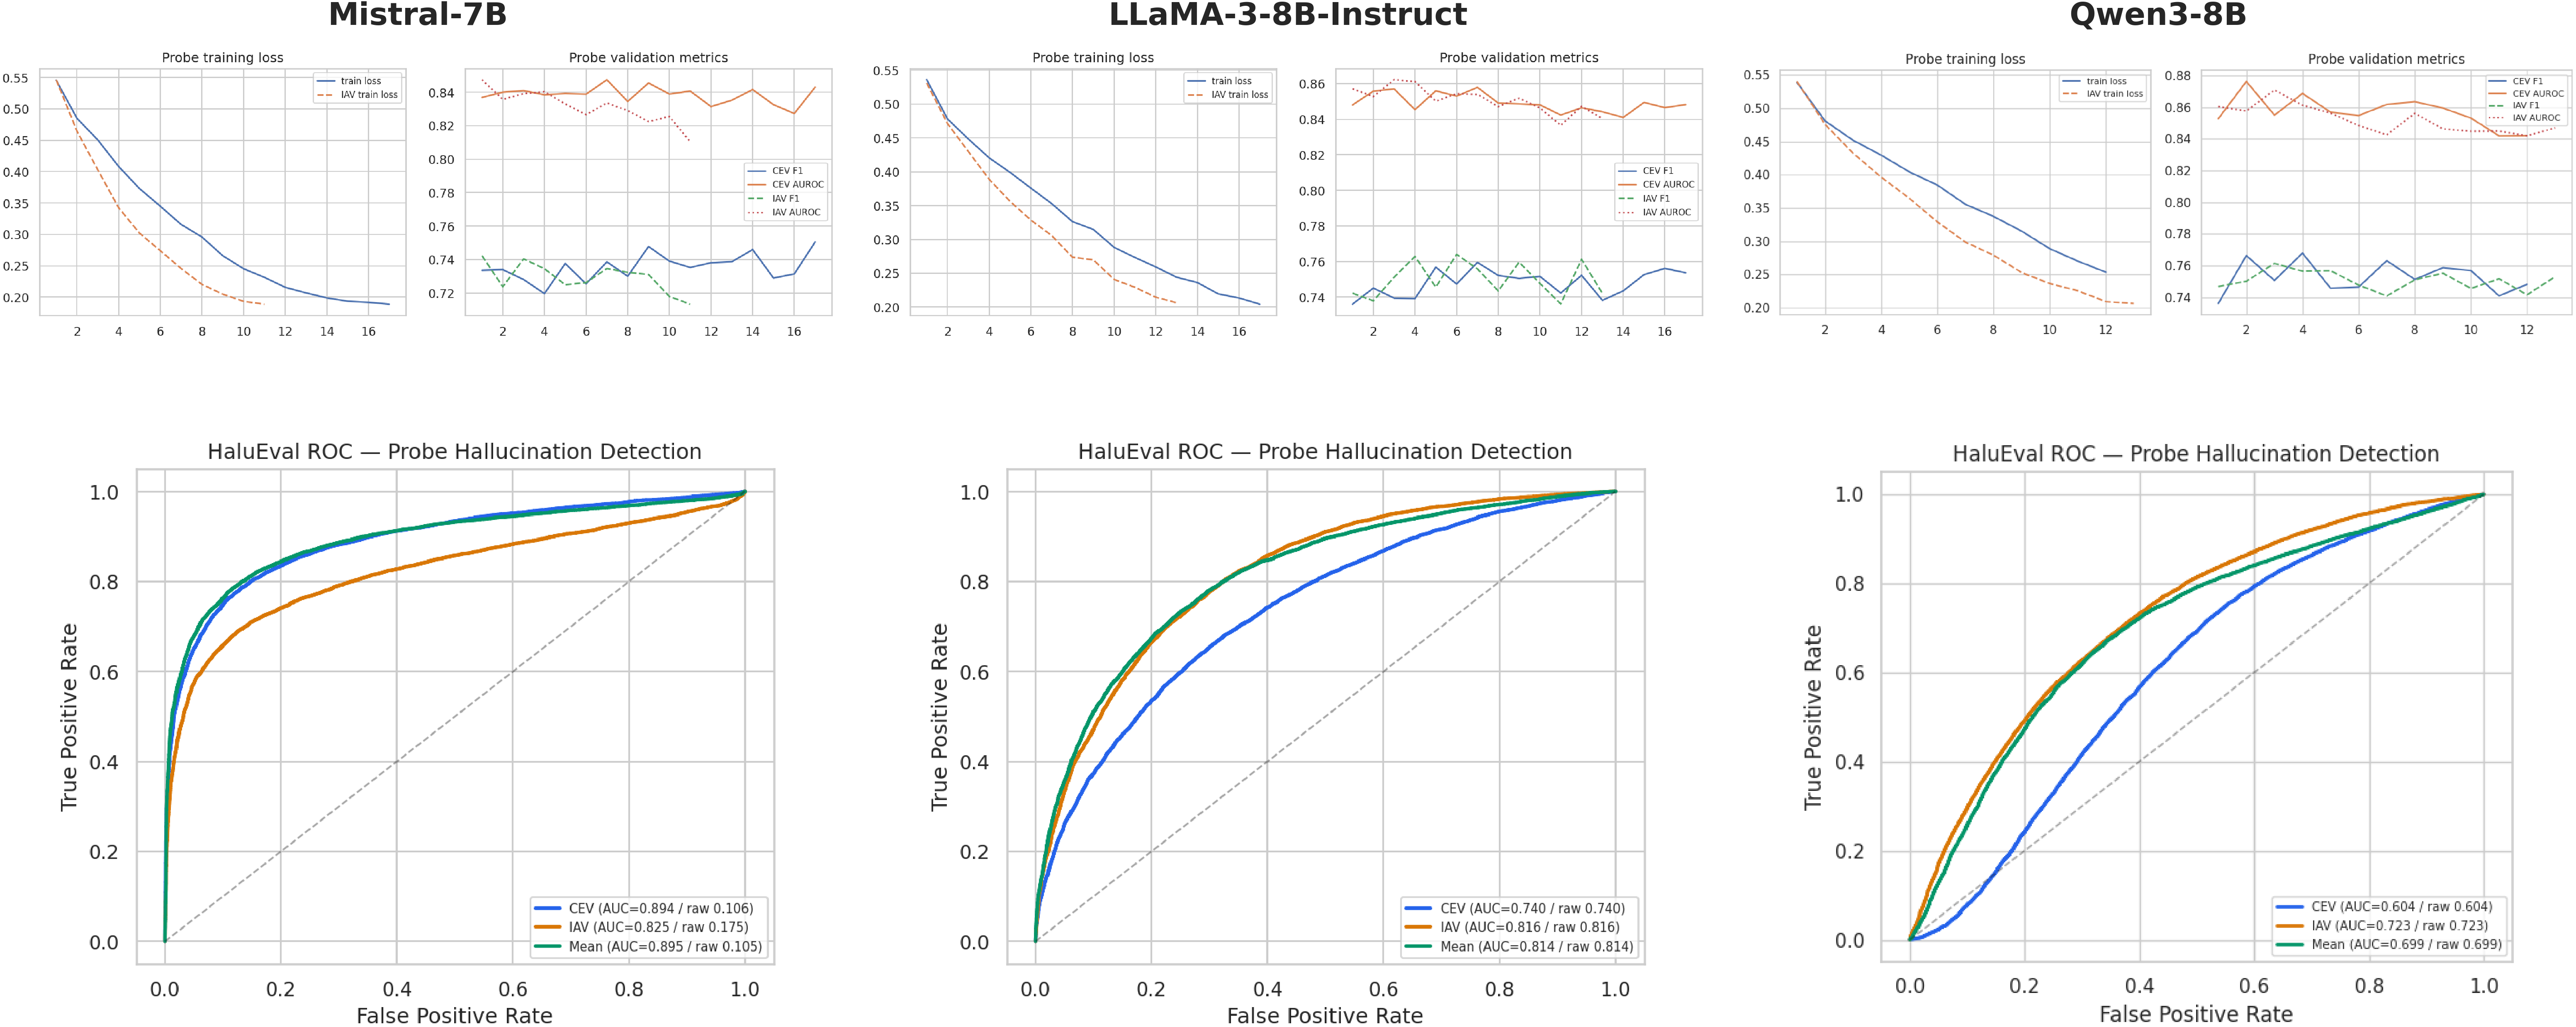
\includegraphics[width=1.05\textwidth]{Images/compare_training_and_halueval_grid.png}
    \caption[Probe training dynamics and HaluEval cross-domain ROC curves.]{Top row: in-domain training loss and validation AUROC for all three backbones. Bottom row: HaluEval out-of-domain ROC curves for CEV, IAV, and fused scores.}
    \label{fig:training_halueval}
\end{figure}

\newpage
\subsection{In-Domain Training Behavior}
\label{sec:indomain_training}

The good news first: training is well-behaved across the board. Loss curves decrease smoothly for both CEV and IAV probes on all three backbones—no instability, no sudden collapses. Validation AUROC climbs and then plateaus, which tells us the probes are learning genuine patterns rather than memorizing training examples.

What is particularly encouraging is that the dual-signal design holds up empirically. IAV tends to be the stronger individual branch, but CEV is never far behind and clearly contributes complementary information. This validates our choice to train two separate probes and fuse them, rather than betting everything on a single signal source.

\subsection{HaluEval Cross-Domain Transfer}
\label{sec:halueval_transfer}

The bottom row of Figure~\ref{fig:training_halueval} is where things get interesting—and, for one backbone, surprising.

For LLaMA-3-8B-Instruct and Qwen3-8B, transfer works as one would hope. The raw AUROC values land above 0.5, meaning the probes trained on RAGTruth still assign higher hallucination scores to the hallucinated HaluEval answers than to the correct ones. The signal generalizes.

Mistral-7B-Instruct-v0.2 is a different story. Its raw AUROC values are far \emph{below} 0.5 around 0.105. At first glance this looks like a catastrophic failure. But look more carefully: an AUROC of 0.105 is not random (which would give 0.5). It means the probe is separating the classes \emph{very well} just in the opposite direction. The adjusted value of $1 - 0.105 = 0.895$ tells us the discriminative power is actually excellent; the polarity just flipped under distribution shift.

The full numerical breakdown is in Table~\ref{tab:halueval_ood} (Section~\ref{sec:halueval_ood}). We do not repeat the numbers here.

\subsection{Interpretation of Mistral Polarity Inversion}
\label{sec:polarity_inversion}

This polarity inversion deserves careful interpretation. It is \emph{not} a bug in the code, if it were random noise, the AUROC would hover around 0.5, not plunge to 0.105. And it is not caused by using a base model instead of an instruction-tuned one; we explicitly use the fully tuned Mistral-7B-Instruct-v0.2 checkpoint.

What seems to be happening is that Mistral's internal representations encode hallucination-relevant information in a way that is directionally specific to the training distribution. When the distribution shifts (from RAGTruth to HaluEval), the \emph{meaning} of certain activation patterns flips. The signal is strong but its sign reverses.

The practical takeaway is sobering but important: \emph{you cannot assume that an internal-state probe will transfer automatically to a new domain, benchmark, or prompt format.} Before deploying in a new setting, the probe needs to be validated and possibly recalibrated on representative examples from the target distribution.

\subsection{Comparison with the Triple-Layer Configuration}
\label{sec:triple_comparison}

One might wonder whether the three-layer concatenation handles distribution shift better than our single mid-layer approach; maybe the extra depth diversity helps with generalization? We checked. It does not.

\begin{figure}[!htb]
    \centering
    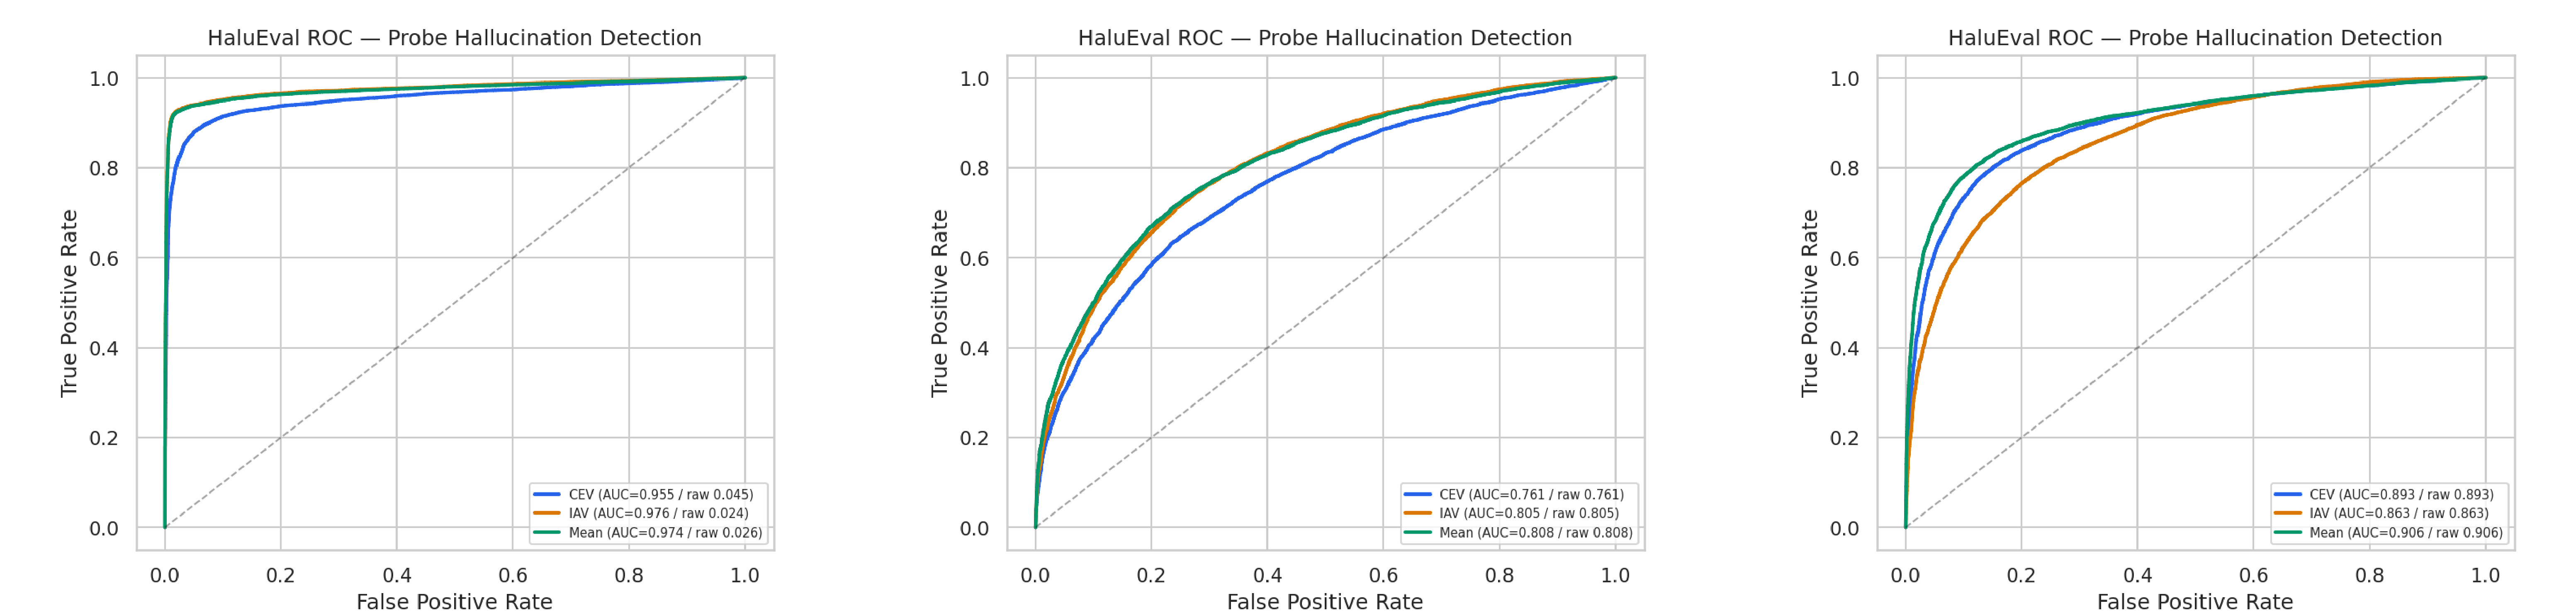
\includegraphics[width=1.00\textwidth]{Images/triple_compare_training_and_halueval_grid.png
}
    \caption[Triple layer Probe training dynamics and HaluEval cross-domain ROC curves.]{Per-backbone HaluEval ROC  for the three-depth (triple) concatenation. }
    \label{fig:Triple layer training_halueval}
\end{figure}



The triple configuration produces nearly identical training curves and HaluEval ROC behavior. Mistral still shows polarity inversion. LLaMA and Qwen still show aligned transfer. No metric meaningfully improves over the single mid-depth result. The extra parameters buy nothing, which further validates the layer-selection decision from Section~\ref{sec:layer_selection}.

%% -------------------------------------------------
\newpage
\section{Post-Training Calibration and Fusion}
\label{sec:calibration_fusion}

Once training is complete, we calibrate each probe independently using temperature scaling:
\begin{equation}
    P(y = 1) = \text{softmax}\!\left(\frac{\mathbf{z}}{T}\right)
\end{equation}

\noindent The temperature $T$ is found by minimizing validation negative log-likelihood. Why bother with this step? Because the controller makes threshold-based decisions. If the probe outputs 0.65 when it really means 0.45, the controller will over-intervene. Calibration ensures that the probability values \emph{mean what they say}.

We calibrate CEV and IAV separately because the two probes can have quite different confidence profiles. One might be well-ranked but systematically overconfident; the other might be better calibrated but with weaker discrimination. Temperature scaling brings them onto a common scale before fusion.

After calibration, the two probabilities are combined:
\[
    p_{\text{fused}} = w \cdot p_{\text{CEV}} + (1 - w) \cdot p_{\text{IAV}}
\]

\noindent with $w$ selected by grid search on the validation split to maximize AUROC. Importantly, this fusion happens at the \emph{probability} level—not by concatenating raw activation vectors into a bigger classifier. Each probe keeps its own learned decision boundary; we combine their judgments, not their inputs.

\begin{table}[!htb]
\centering
\caption{Calibration and fusion settings.}
\label{tab:calibration_settings}
\begin{tabular}{@{}ll@{}}
\toprule
\textbf{Component} & \textbf{Setting} \\
\midrule
Calibration method        & Temperature scaling \\
Calibration scope         & Applied separately to CEV and IAV probes \\
Calibration objective     & Minimize validation NLL \\
Fusion type               & Probability-level convex fusion \\
Fusion formula            & $p_{\text{fused}} = w \cdot p_{\text{CEV}} + (1-w) \cdot p_{\text{IAV}}$ \\
Fusion weight selection   & Validation-set grid search \\
Fusion objective          & Maximize validation AUROC \\
Controller input          & $p_{\text{fused}}$ \\
\bottomrule
\end{tabular}
\end{table}

%% -------------------------------------------------
\newpage
\section{Summary}
\label{sec:ch6_summary}

What have we learned in this chapter? Three things stand out.

First, the probes train stably and learn true hallucination-relevant patterns on RAGTruth both CEV and IAV converge smoothly, and validation metrics confirm generalization to the held-out split.

Second, the out-of-domain transfer is real but model dependent. Qwen3-8B and LLaMA-3-8B-Instruct still perform well in their discriminative manner on HaluEval. Mistral-7B-Instruct-v0.2 is still very discriminative, but the polarity is reversed, an interesting result showing how sensitive these probes can be to the distribution.

Third, calibration is not an option. The downstream controller makes absolute threshold decisions, so the probes need to produce probabilities associated with empirical risk levels. This is achieved with temperature scaling and probability-level fusion, which keeps the two signals separate but combines their strengths.

The bottom line is that internal-state probes are effective, but they are not plug-and-play across domains. Deploy with confidence. Validate first.


% =====================================================
% REFERENCES
% =====================================================

\clearpage
\singlespacing

\bibliographystyle{IEEEtran}
\bibliography{ref}

% =====================================================
% APPENDIX
% =====================================================

\clearpage
\clearpage
\appendix

% ------ Appendix Heading ------
\chapter*{Appendices}
\addcontentsline{toc}{chapter}{Appendices}
\markboth{Appendices}{Appendices}

\vspace{0.8cm}

% ------ Appendix A ------
\begin{center}
\textbf{Appendix A: [Title of First Appendix]}
\end{center}

\vspace{0.5cm}

\noindent Start each appendix on a new page. Place appendices in the same order as they are referred to in the body of the Thesis. That is, the first appendix referred to should be Appendix A, the second appendix referred to should be Appendix B, and so on. Appendix formatting can be different to the main document. Refer to \textit{Thesis PAM} for information about appendix figures and tables.

\vspace{1cm}

% ------ Appendix B ------
\begin{center}
\textbf{Appendix B: [Title of First Appendix]}
\end{center}

\vspace{0.8cm}

% ------ Appendix C ------
\begin{center}
\textbf{Appendix C: [Title of First Appendix]}
\end{center}

\end{document}